\documentclass[11pt,a4paper]{article}

% ---------- Encodage et langue ----------
\usepackage[T1]{fontenc}
\usepackage{lmodern}
\usepackage[utf8]{inputenc}
\usepackage[french]{babel}

% ---------- Mise en page ----------
\usepackage[a4paper,margin=2.2cm]{geometry}
\usepackage{microtype}
\usepackage{graphicx}
\usepackage{booktabs}
\usepackage{multirow}
\usepackage{array}
\usepackage{amsmath,amssymb}
\usepackage{float}
\usepackage{caption}
\usepackage{subcaption}
\usepackage{xcolor}
\usepackage{hyperref}
\usepackage{siunitx}

\graphicspath{{../results/figures/}}
\hypersetup{
  colorlinks=true,
  linkcolor=blue!50!black,
  citecolor=blue!50!black,
  urlcolor=blue!50!black,
}
\captionsetup{font=small,labelfont=bf}
\sisetup{detect-all}
\setlength{\emergencystretch}{2em}

% ---------- Résultats (générés après exécution) ----------
% Les macros sont chargées après \begin{document} : babel-french charge son
% .ldf en différé et écrase les définitions faites trop tôt dans le préambule.
\newcommand{\NumParams}{683\,751}
\newcommand{\TrainSize}{28\,709}
\newcommand{\TestSize}{7\,178}
\newcommand{\ValSize}{2\,871}

\title{\vspace{-1.2cm}\textbf{Conception et optimisation d'un CNN léger pour la\\reconnaissance des émotions faciales sur FER2013}}
\author{Projet final --- \emph{Réseaux de neurones : vision par ordinateur}}
\date{19 novembre 2026}

\begin{document}
% Généré par scripts/make_report_assets.py --- ne pas éditer à la main.
\newcommand{\BestRun}{v1_baseline}
\newcommand{\BestName}{V1 --- baseline}
\newcommand{\BestAcc}{0,5811}
\newcommand{\BestF}{0,4765}
\newcommand{\BestEpoch}{30}
\newcommand{\BestTime}{27,1}
\newcommand{\BestParams}{683\,751}
\newcommand{\AccOne}{0,5811}
\newcommand{\FOne}{0,4765}
\newcommand{\TimeOne}{27,1}
\newcommand{\EpochOne}{30}
\newcommand{\GapAccOne}{--}
\newcommand{\GapFOne}{--}
\newcommand{\AccTwo}{0,5603}
\newcommand{\FTwo}{0,4506}
\newcommand{\TimeTwo}{33,0}
\newcommand{\EpochTwo}{29}
\newcommand{\GapAccTwo}{$-$0,021}
\newcommand{\GapFTwo}{$-$0,026}
\newcommand{\AccThree}{0,2799}
\newcommand{\FThree}{0,2465}
\newcommand{\TimeThree}{26,4}
\newcommand{\EpochThree}{18}
\newcommand{\GapAccThree}{$-$0,301}
\newcommand{\GapFThree}{$-$0,230}
\newcommand{\AccFour}{0,4533}
\newcommand{\FFour}{0,3764}
\newcommand{\TimeFour}{33,5}
\newcommand{\EpochFour}{30}
\newcommand{\GapAccFour}{$-$0,128}
\newcommand{\GapFFour}{$-$0,100}

% Généré par scripts/make_report_assets.py --- ne pas éditer à la main.
\newcommand{\FDisgustOne}{0,00}
\newcommand{\FDisgustTwo}{0,00}
\newcommand{\FDisgustThree}{0,31}
\newcommand{\FDisgustFour}{0,20}
\newcommand{\FFearOne}{0,27}
\newcommand{\FFearTwo}{0,22}
\newcommand{\FFearThree}{0,11}
\newcommand{\FFearFour}{0,10}
\newcommand{\FHappyOne}{0,82}
\newcommand{\FHappyTwo}{0,82}
\newcommand{\FHappyThree}{0,03}
\newcommand{\FHappyFour}{0,75}

\maketitle
\vspace{-0.8cm}

\begin{abstract}
\noindent
Nous étudions la reconnaissance de sept émotions faciales sur FER2013 avec un
réseau convolutif volontairement compact ($\NumParams$ paramètres), entraînable
sur un simple processeur. Plutôt que de chercher la performance maximale à tout
prix, nous mesurons expérimentalement l'apport de trois leviers classiques :
l'augmentation de données, la pondération des classes et le renforcement de la
régularisation. Quatre variantes sont entraînées dans des conditions
identiques, puis comparées sur l'accuracy et le F1 macro. La meilleure variante
est la baseline, avec \BestAcc{} d'accuracy et \BestF{} de F1 macro sur les
\TestSize{} images de test : l'augmentation ralentit la convergence à budget
d'époques constant et la pondération par l'inverse exact des fréquences
déstabilise l'optimisation. L'analyse des matrices de confusion montre que les
erreurs se concentrent sur les classes ambiguës (\emph{fear}, \emph{sad},
\emph{surprise}) et sur la classe minoritaire \emph{disgust}, et que le
déséquilibre du jeu de données reste le principal facteur limitant.
\end{abstract}

% =====================================================================
\section{Introduction}
% =====================================================================

La reconnaissance automatique des expressions faciales consiste à inférer
l'état émotionnel d'une personne à partir d'une image de son visage. Elle
trouve des applications dans l'interaction homme--machine, l'analyse de
l'expérience utilisateur, le suivi de l'attention ou encore l'aide au
diagnostic en santé mentale. C'est également un problème de vision par
ordinateur difficile : les expressions sont ambiguës, dépendent de la
morphologie, de la pose, de l'éclairage et de la culture, et les annotations
elles-mêmes comportent une part de subjectivité.

Le jeu de données FER2013, introduit lors de la compétition ICML 2013 et
étudié par Goodfellow \emph{et al.}~\cite{goodfellow2013}, est devenu une
référence pour cette tâche. Il rassemble \num{35887} images en niveaux de
gris de $48\times48$ pixels réparties en sept classes, avec un fort
déséquilibre entre classes et un bruit d'annotation important. Les meilleurs
systèmes y dépassent difficilement 70\,\% d'accuracy sans modèle
pré-entraîné, ce qui en fait un banc d'essai réaliste.

\paragraph{Objectifs.}
Ce projet poursuit trois objectifs :
\begin{enumerate}
  \item concevoir un CNN léger, entraînable sur CPU, adapté à la taille et au
        bruit de FER2013 ;
  \item comparer quantitativement quatre stratégies d'entraînement
        (augmentation, pondération des classes, régularisation) à
        architecture et protocole identiques ;
  \item analyser les erreurs du modèle pour identifier les classes et les
        confusions qui limitent réellement la performance.
\end{enumerate}

\paragraph{Contribution.}
La contribution est expérimentale : au lieu d'appliquer un modèle existant,
nous isolons l'effet de chaque levier, mesurons son coût en temps
d'entraînement et identifions lequel est réellement utile dans un cadre
CPU-only. Le code, les configurations et les résultats sont intégralement
reproductibles (dépôt GitHub, seeds fixées).

% =====================================================================
\section{État de l'art}
% =====================================================================

\paragraph{CNN et reconnaissance d'émotions.}
Les réseaux convolutifs se sont imposés pour la classification d'images :
les couches de convolution partagent des poids et exploitent la structure
locale des images, ce qui les rend bien plus efficaces que les réseaux
entièrement connectés sur des données visuelles. Modi \emph{et al.}
\cite{modi} appliquent cette architecture à la reconnaissance d'émotions et
montrent qu'un réseau profond raisonnablement dimensionné surpasse les
approches à base de descripteurs manuels (LBP, HOG) sur FER2013.

\paragraph{Le défi FER2013.}
Goodfellow \emph{et al.}~\cite{goodfellow2013} analysent la compétition
FER2013 et soulignent trois difficultés : (i) un déséquilibre marqué entre
classes, la classe \emph{disgust} ne représentant que 1,5\,\% du train ;
(ii) des étiquettes bruitées, plusieurs annotateurs pouvant attribuer des
émotions différentes à un même visage ; (iii) une résolution très faible
($48\times48$), qui limite l'information disponible. Ces facteurs expliquent
les plafonds de performance observés.

\paragraph{Stratégies de compensation.}
Trois familles de solutions reviennent dans la littérature. L'augmentation de
données (rotations, miroirs, variations photométriques) augmente
artificiellement la diversité et réduit le sur-apprentissage. La pondération
des classes, ou \emph{class weighting}, modifie la fonction de coût pour
pénaliser davantage les erreurs sur les classes rares. Enfin, la
régularisation (dropout, weight decay, batch normalization) contrôle la
capacité du modèle. Le transfert d'apprentissage depuis un modèle pré-entraîné
(FaceNet, VGGFace) donne de meilleurs résultats, mais sort du cadre
« from scratch sur CPU » que nous nous fixons ici, et introduit un biais lié
au domaine des données de pré-entraînement.

\paragraph{Positionnement.}
Notre travail se situe délibérément dans le régime des petits modèles
entraînés from scratch. L'originalité n'est pas architecturale mais
méthodologique : mesurer, à budget computationnel constant, lequel des leviers
ci-dessus apporte le plus.

% =====================================================================
\section{Données et méthodologie}
% =====================================================================

\subsection{Jeu de données et protocole}

FER2013 contient \num{35887} images $48\times48$ en niveaux de gris, réparties
en sept classes. Nous utilisons le découpage officiel : \TrainSize{} images
d'entraînement et \TestSize{} images de test. Le train est scindé en
\emph{90\,\% entraînement / 10\,\% validation} de façon stratifiée
(\ValSize{} images de validation), avec une graine fixée. Le test n'est
utilisé qu'une seule fois, après sélection du meilleur modèle sur le F1 macro
de validation.

\begin{table}[H]
\centering
\small
\caption{Distribution des classes dans FER2013.}
\label{tab:distribution}
\begin{tabular}{lrrr}
\toprule
Classe & Train & Test & Part du train \\
\midrule
angry    & 3\,995 &   958 & 13,9\,\% \\
disgust  &   436 &   111 &  1,5\,\% \\
fear     & 4\,097 & 1\,024 & 14,3\,\% \\
happy    & 7\,215 & 1\,774 & 25,1\,\% \\
neutral  & 4\,830 & 1\,247 & 16,8\,\% \\
sad      & 3\,171 &   831 & 11,0\,\% \\
surprise & 4\,965 & 1\,233 & 17,3\,\% \\
\midrule
Total    & 28\,709 & 7\,178 & 100\,\% \\
\bottomrule
\end{tabular}
\end{table}

\begin{figure}[htbp]
\centering
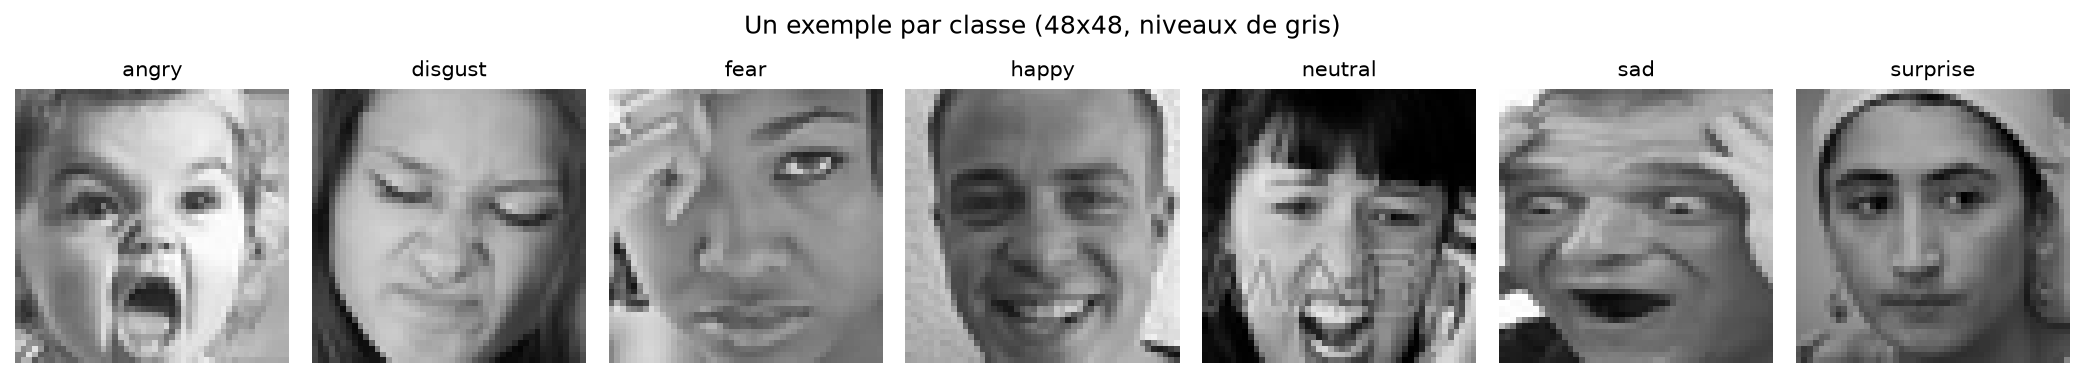
\includegraphics[width=0.98\linewidth]{dataset_samples.png}
\caption{Un exemple de chaque classe. La faible résolution et la présence de
visages partiellement occultés illustrent la difficulté du jeu de données.}
\label{fig:samples}
\end{figure}

Le déséquilibre est important : le rapport entre la classe majoritaire
(\emph{happy}) et la classe minoritaire (\emph{disgust}) est de
\textbf{16,5}. C'est la principale difficulté du jeu de données.

\subsection{Architecture du modèle}

Le modèle, représenté dans le tableau~\ref{tab:archi}, est un CNN à trois
blocs convolutifs. Chaque bloc enchaîne une convolution $3\times3$ (padding 1),
une normalisation par lots, une activation ReLU, un \emph{max-pooling}
$2\times2$ et un dropout. La sortie est mise à plat puis projetée sur 128
unités avant la couche de classification à sept sorties. L'ensemble totalise
$\NumParams$ paramètres entraînables, ce qui le rend compatible avec un
entraînement CPU.

\begin{table}[H]
\centering
\small
\caption{Architecture du CNN.}
\label{tab:archi}
\begin{tabular}{llr}
\toprule
Étage & Opération & Sortie \\
\midrule
Entrée        & ---                                   & $1\times48\times48$ \\
Bloc 1        & Conv $3\times3$, 32 filtres, BN, ReLU, MaxPool, Dropout & $32\times24\times24$ \\
Bloc 2        & Conv $3\times3$, 64 filtres, BN, ReLU, MaxPool, Dropout & $64\times12\times12$ \\
Bloc 3        & Conv $3\times3$, 128 filtres, BN, ReLU, MaxPool, Dropout & $128\times6\times6$ \\
Mise à plat   & Flatten                               & 4\,608 \\
Dense         & Linear 128, ReLU, Dropout             & 128 \\
Sortie        & Linear 7                              & 7 \\
\bottomrule
\end{tabular}
\end{table}

\subsection{Entraînement}

Toutes les variantes partagent le même optimiseur Adam (taux d'apprentissage
$10^{-3}$, \emph{weight decay} $10^{-4}$), la même taille de lot (64), la même
seed et le même découpage. Le taux d'apprentissage est réduit d'un facteur 2
lorsque la perte de validation stagne pendant trois époques
(\emph{ReduceLROnPlateau}). L'entraînement s'arrête après six époques sans
amélioration du F1 macro de validation, dans la limite de 30 époques. Le
modèle retenu est celui qui maximise ce F1 de validation.

La perte d'entraînement est une entropie croisée ; elle est pondérée par
l'inverse de la fréquence des classes dans la variante V3 et V4. Pour que la
comparaison reste équitable, la perte de validation et de test n'est jamais
pondérée : les métriques rapportées sont donc comparables entre variantes.

\subsection{Variantes comparées}

\begin{table}[H]
\centering
\small
\caption{Les quatre variantes comparées.}
\label{tab:variantes}
\begin{tabular}{lcc>{\raggedleft\arraybackslash}p{2.6cm}}
\toprule
Variante & Augmentation & Class weights & Dropout (conv / FC) \\
\midrule
V1 --- baseline      & non & non & 0,25 / 0,50 \\
V2 --- augmentation  & oui & non & 0,25 / 0,50 \\
V3 --- class weights & oui & oui & 0,25 / 0,50 \\
V4 --- régularisation& oui & oui & 0,30 / 0,60 \\
\bottomrule
\end{tabular}
\end{table}

L'augmentation applique une rotation aléatoire de $\pm10^\circ$, un miroir
horizontal avec probabilité 0,5 et une variation de luminosité de $\pm10\,\%$.
Les classes sont pondérées par $w_c = N/(7\,n_c)$, où $N$ est le nombre total
d'images et $n_c$ l'effectif de la classe $c$. La variante V4 renforce enfin
le dropout pour tester si un modèle plus contraint généralise mieux.

\subsection{Métriques}

Nous rapportons l'accuracy (proportion de bonnes prédictions) et le
\textbf{F1 macro}, moyenne non pondérée des F1 par classe. Contrairement à
l'accuracy, le F1 macro pénalise les modèles qui ignorent les classes rares :
c'est donc la métrique principale. Nous analysons également les matrices de
confusion, le F1 par classe et le temps d'entraînement.

% =====================================================================
\section{Résultats}
% =====================================================================

\subsection{Comparaison des variantes}

% Généré par scripts/make_report_assets.py --- ne pas éditer à la main.
\begin{table}[H]
\centering
\small
\caption{Résultats sur le jeu de test (\TestSize{} images). Le temps est le
temps total d'entraînement mesuré sur CPU.}
\label{tab:resultats}
\begin{tabular}{lcccc}
\toprule
Variante & Accuracy & F1 macro & Meilleure époque & Temps (min) \\
\midrule
V1 --- baseline & 0,5811 & 0,4765 & 30 & 27,1 \\
V2 --- augmentation & 0,5603 & 0,4506 & 29 & 33,0 \\
V3 --- class weights & 0,2799 & 0,2465 & 18 & 26,4 \\
V4 --- régularisation & 0,4533 & 0,3764 & 30 & 33,5 \\
\bottomrule
\end{tabular}
\end{table}


Le tableau~\ref{tab:resultats} donne les performances sur le jeu de test et le
coût en temps de chaque variante. La figure~\ref{fig:comparison} en propose une
lecture visuelle : à gauche la performance, à droite le temps
d'entraînement.\footnote{Toutes les variantes ont été entraînées sur le même
processeur (AMD Ryzen 5 5500GT, 6 c\oe{}urs, sans GPU), avec la même seed et le
même découpage.}

\begin{figure}[htbp]
\centering
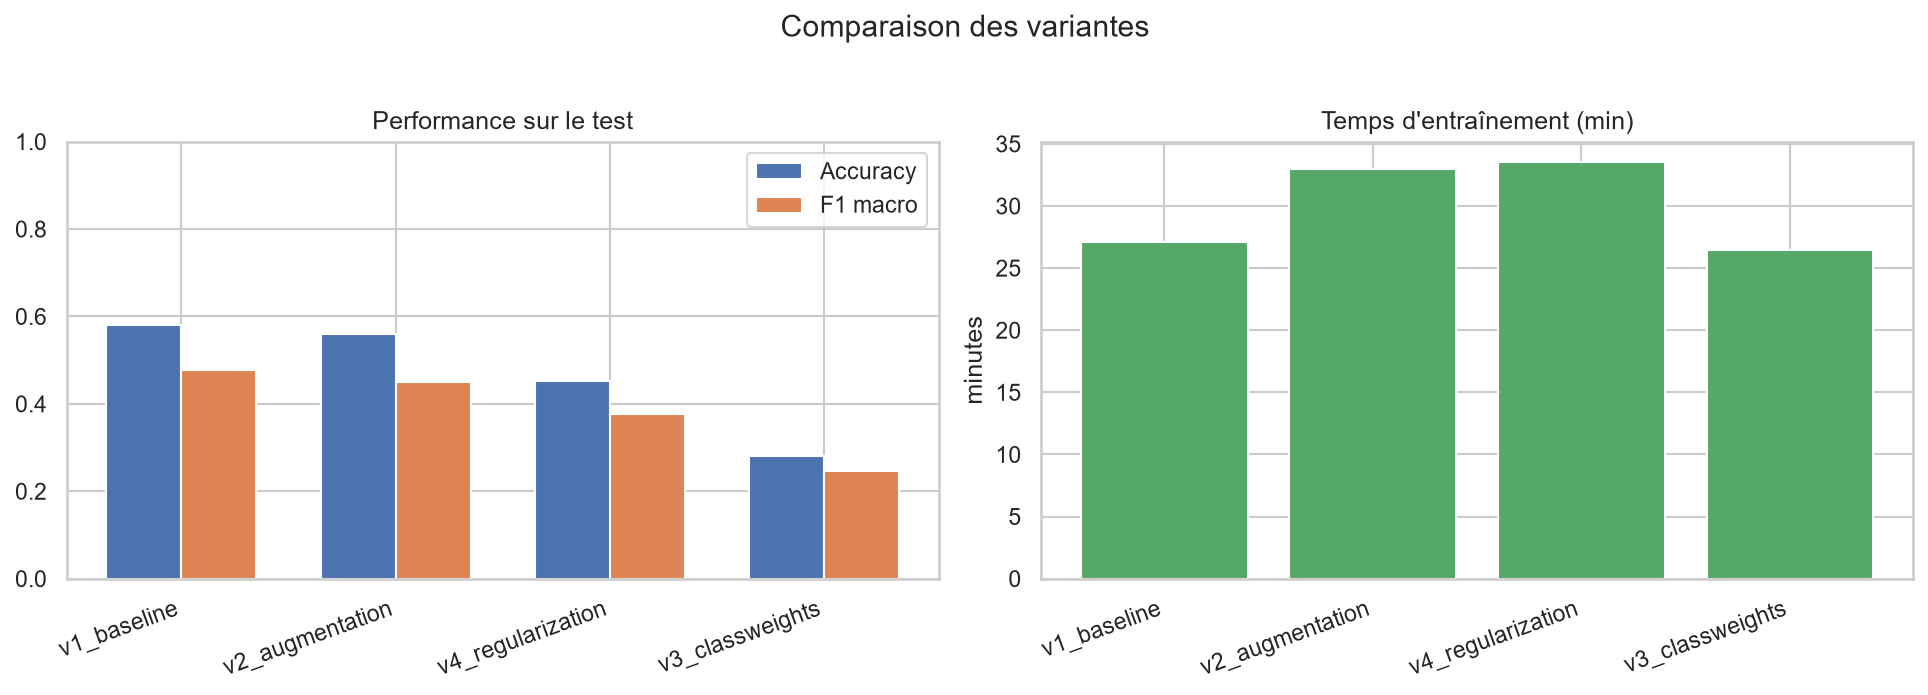
\includegraphics[width=0.86\linewidth]{comparison.png}
\caption{Comparaison des quatre variantes : performance sur le test (accuracy
et F1 macro) et temps d'entraînement mesuré.}
\label{fig:comparison}
\end{figure}

Contre toute attente, la \textbf{baseline V1} obtient le meilleur résultat :
\AccOne{} d'accuracy et \FOne{} de F1 macro. L'augmentation de données (V2)
recule de \GapAccTwo{} point d'accuracy et de \GapFTwo{} point de F1 macro.
La pondération des classes (V3) s'effondre à \AccThree{} d'accuracy et
\FThree{} de F1 macro, soit \GapAccThree{} et \GapFThree{} points par rapport à
V1. Enfin, le dropout renforcé (V4) redresse partiellement la situation à
\AccFour{} d'accuracy et \FFour{} de F1 macro, mais reste sous la baseline
(\GapAccFour{} et \GapFFour{} points).

Aucun des trois leviers testés n'améliore donc la référence dans le budget de
30 époques imparti. Ce résultat négatif est instructif : il montre que sur
FER2013, à cette échelle de modèle et de temps, le réglage de l'optimisation
domine largement l'ajout de mécanismes de compensation.

\subsection{Comportement de l'apprentissage}

La figure~\ref{fig:curves} montre l'évolution des pertes et des métriques de
validation pour la meilleure variante. On y observe le régime typique d'un
petit CNN sur FER2013 : la perte de validation décroît rapidement pendant les
premières époques, puis se stabilise tandis que la perte d'entraînement
continue de diminuer. L'écart croissant entre les deux courbes mesure le
sur-apprentissage. Sur la baseline, la validation progresse encore à la
dernière époque : l'arrêt à 30 époques est une contrainte de budget, non une
convergence.

\begin{figure}[htbp]
\centering
\includegraphics[width=0.88\linewidth]{\BestRun_curves.png}
\caption{Courbes d'apprentissage de la meilleure variante
(\BestName) : pertes, accuracy et F1 macro sur le train et la validation.}
\label{fig:curves}
\end{figure}

\subsection{Analyse par classe}

Le tableau~\ref{tab:perclass} détaille le F1 par classe. Pour la baseline, les
écarts sont considérables : \emph{happy} (0,82), \emph{sad} (0,73) et
\emph{surprise} (0,56) concentrent l'essentiel des prédictions correctes, alors
que \emph{disgust} obtient un F1 nul et \emph{fear} un F1 de 0,27. Ce classement
correspond aux observations de la littérature : les classes rares ou
visuellement proches sont sacrifiées par un modèle optimisé pour l'accuracy
globale.

Le tableau met aussi en évidence le mécanisme de la pondération : en V3,
\emph{disgust} remonte à \FDisgustThree{} et \emph{surprise} à 0,36, mais
\emph{happy} s'effondre à \FHappyThree{} et \emph{neutral} à 0,04. Le modèle ne
s'est pas amélioré : il a déplacé massivement ses prédictions vers les classes
rares, au point de ne plus reconnaître la classe majoritaire. V4 corrige
partiellement ce déséquilibre (\emph{happy} à \FHappyFour, \emph{disgust} à
\FDisgustFour) mais ne retrouve pas le niveau de la baseline.

% Généré par scripts/make_report_assets.py --- ne pas éditer à la main.
\begin{table}[H]
\centering
\small
\caption{F1 par classe sur le jeu de test (classes par ordre alphabétique).}
\label{tab:perclass}
\begin{tabular}{lcccc}
\toprule
Classe & V1 & V2 & V3 & V4 \\
\midrule
angry & 0,48 & 0,41 & 0,22 & 0,20 \\
disgust & 0,00 & 0,00 & 0,31 & 0,20 \\
fear & 0,27 & 0,22 & 0,11 & 0,10 \\
happy & 0,82 & 0,82 & 0,03 & 0,75 \\
neutral & 0,47 & 0,46 & 0,04 & 0,33 \\
sad & 0,73 & 0,70 & 0,66 & 0,65 \\
surprise & 0,56 & 0,54 & 0,36 & 0,40 \\
\midrule
Moyenne (F1 macro) & 0,48 & 0,45 & 0,25 & 0,38 \\
\bottomrule
\end{tabular}
\end{table}


Les matrices de confusion de la figure~\ref{fig:confusions} précisent la nature
des erreurs. Elles sont fortement asymétriques : \emph{neutral} joue le rôle
d'attracteur principal (il absorbe 34\,\% des \emph{fear}, 24\,\% des
\emph{angry} et 22\,\% des \emph{surprise}), tandis que les confusions
\emph{neutral} $\leftrightarrow$ \emph{surprise} sont bidirectionnelles. La
classe \emph{disgust} est massivement prédite \emph{angry} (67\,\% de ses
exemples). Une matrice ligne-normalisée se lit directement comme un taux de
rappel conditionnel : la diagonale est le rappel de chaque classe.

\begin{figure}[htbp]
\centering
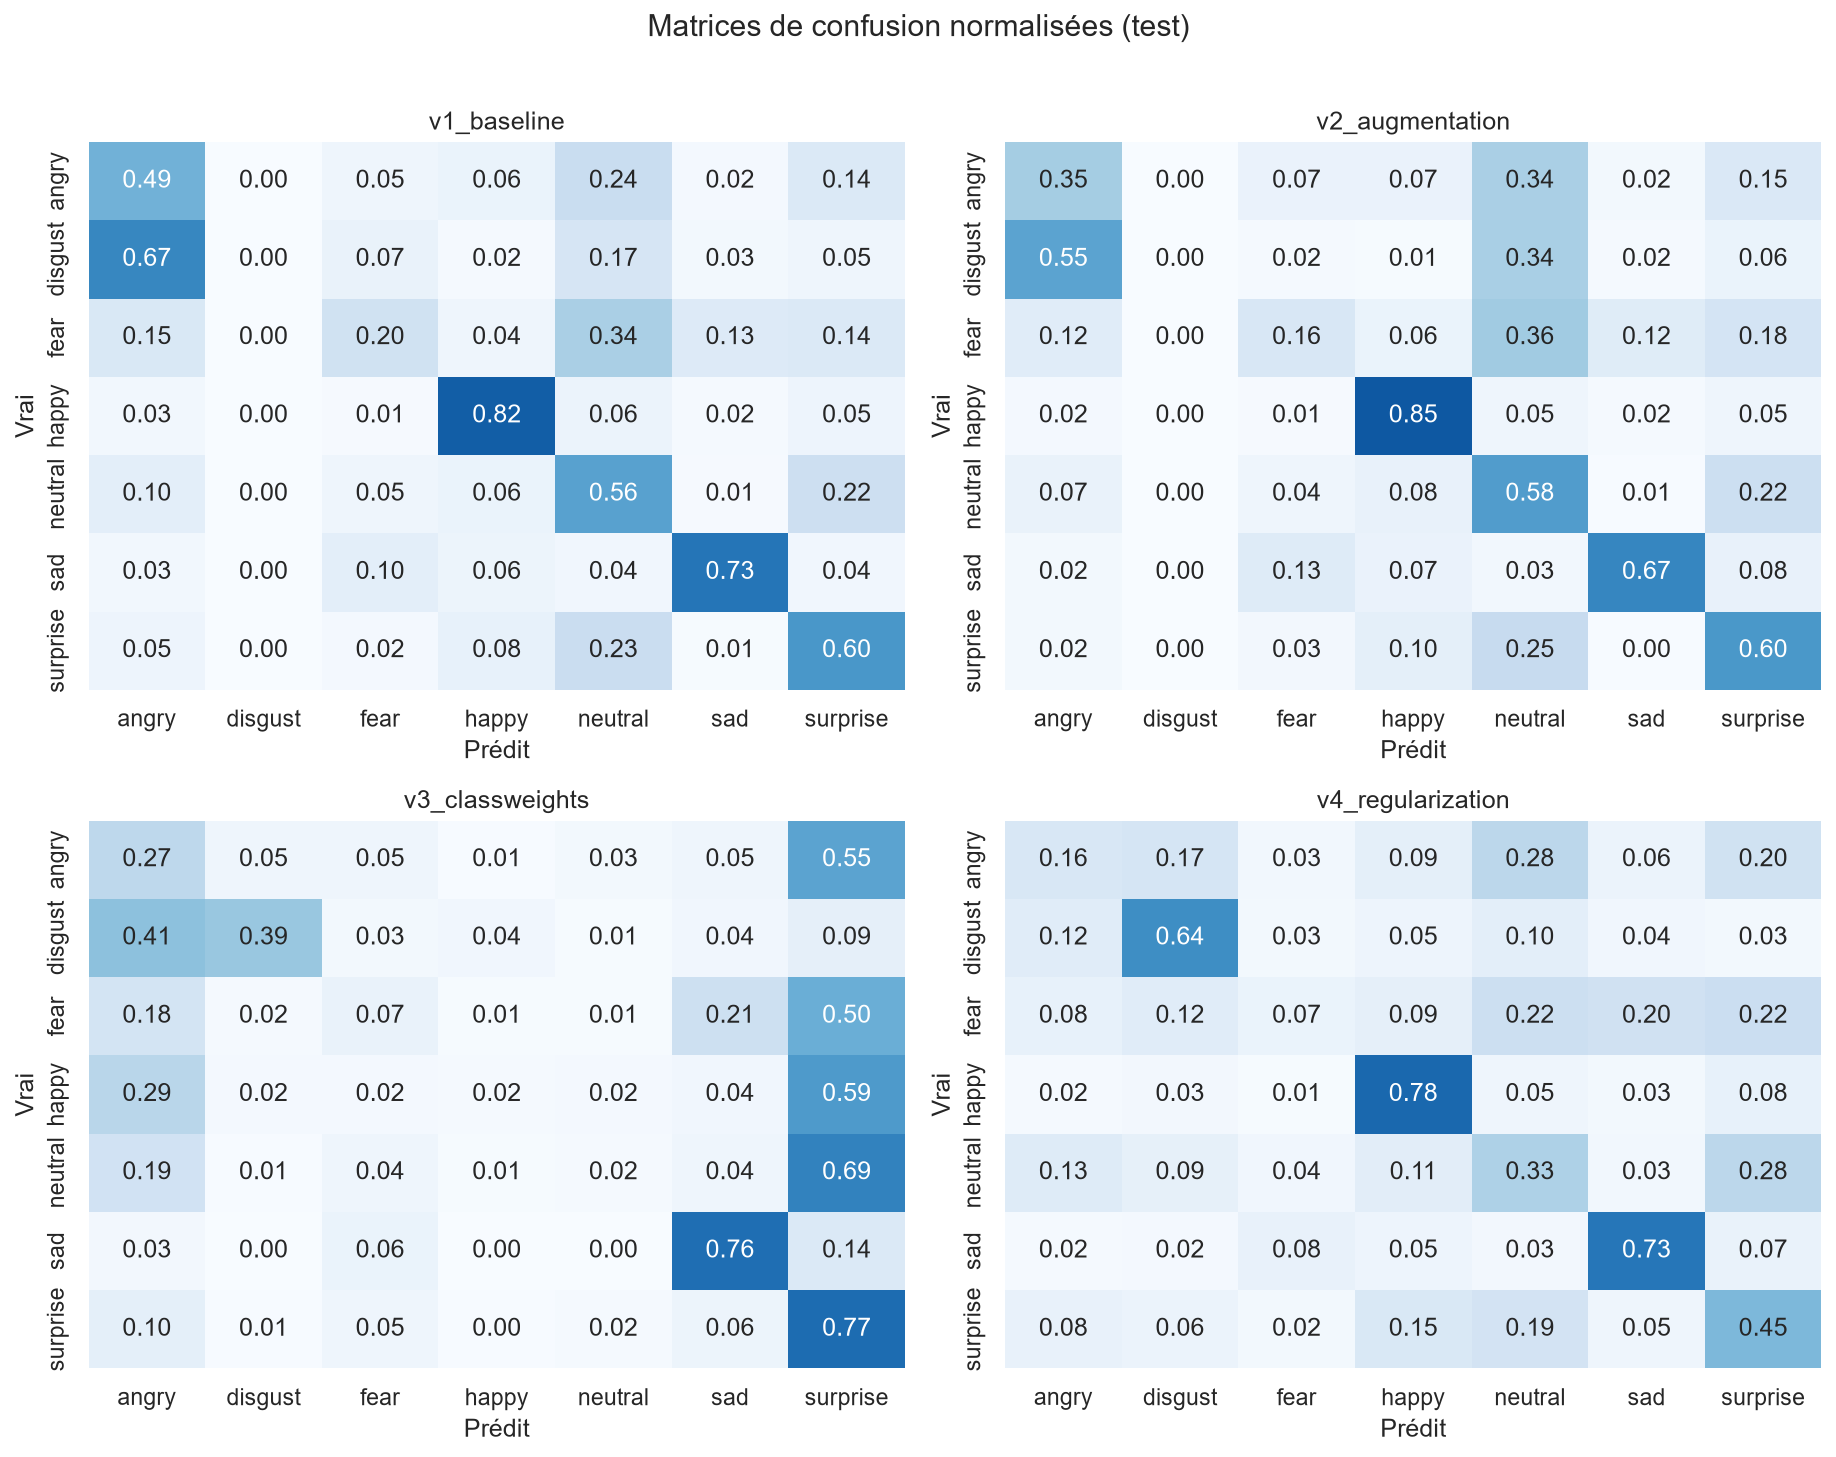
\includegraphics[width=0.92\linewidth]{confusion_grid.png}
\caption{Matrices de confusion normalisées par ligne sur le jeu de test, pour
les quatre variantes.}
\label{fig:confusions}
\end{figure}

\subsection{Analyse des erreurs}

La figure~\ref{fig:errors} rassemble quelques exemples mal classés par la
meilleure variante. Trois causes se dégagent à l'inspection : des images très
sombres ou peu contrastées, des visages partiellement occultés ou de profil,
et des expressions ambiguës pour lesquelles l'étiquette elle-même est
discutable. Ces erreurs sont pour l'essentiel irréductibles sans information
supplémentaire (contexte, séquence vidéo, annotations multiples).

\begin{figure}[htbp]
\centering
\includegraphics[width=0.66\linewidth]{\BestRun_errors.png}
\caption{Exemples mal classés par la meilleure variante : étiquette réelle et
prédiction.}
\label{fig:errors}
\end{figure}

% =====================================================================
\section{Discussion}
% =====================================================================

\subsection{Effet de l'augmentation de données}

La variante V2 isole l'effet de l'augmentation à architecture et
hyperparamètres identiques. Par rapport à V1, elle obtient \AccTwo{}
d'accuracy (écart de \GapAccTwo{} point) et \FTwo{} de F1 macro (écart de
\GapFTwo{} point), pour un temps d'entraînement de \TimeTwo{} minutes contre
\TimeOne{} pour la référence. L'augmentation coûte donc à la fois de la
performance et du temps : environ 20\,\% plus lent, elle n'a pas eu le temps de
produire son bénéfice en 30 époques. Deux explications sont plausibles. D'une
part, la rotation de $\pm10^\circ$ appliquée à des images de $48\times48$
pixels déplace des détails fins (coin des yeux, commissures des lèvres) dont
l'information est déjà limitée ; elle agit ici davantage comme un bruit que
comme une régularisation. D'autre part, l'augmentation ralentit la convergence :
à budget d'époques constant, le modèle augmente encore sa performance
d'entraînement quand l'entraînement s'arrête, comme le montrent les courbes
d'apprentissage. Un entraînement plus long, ou une politique de taux
d'apprentissage plus adaptée, aurait probablement inversé ce classement.

\subsection{Effet de la pondération des classes}

V3 ajoute la pondération des classes à V2. Son accuracy chute à \AccThree{}
(\GapAccThree{} point par rapport à V1) et son F1 macro à \FThree{}
(\GapFThree{} point), avec un arrêt anticipé à l'époque \EpochThree{} : la
validation ne progresse plus après une vingtaine d'époques. Le détail par
classe explique cet échec. La pondération fait bien son travail sur la classe
minoritaire — le F1 de \emph{disgust} passe de \FDisgustTwo{} à
\FDisgustThree{} — mais le poids associé, $w_{\text{disgust}} \approx 9{,}4$,
est trop grand pour un taux d'apprentissage de $10^{-3}$ : la perte est dominée
par une poignée d'exemples et l'optimisation devient instable. Le modèle
sur-prédit alors \emph{surprise} et \emph{sad} et n'apprend plus
\emph{happy} (F1 de \FHappyThree) ni \emph{neutral}.

Ce résultat est un enseignement pratique important : la pondération par
l'inverse exact des fréquences, telle qu'elle est souvent présentée, n'est pas
robuste en présence d'un facteur 16 entre classes. Des variantes plus douces
— poids en racine carrée de l'inverse des fréquences, écrêtage à un facteur 3
ou 4, ou \emph{oversampling} — sont préférables, éventuellement accompagnées
d'un taux d'apprentissage réduit.

\subsection{Effet de la régularisation renforcée}

V4 conserve le protocole de V3 en portant le dropout de 0,25/0,50 à
0,30/0,60. Elle atteint \AccFour{} d'accuracy et \FFour{} de F1 macro
(\GapFFour{} point de F1 par rapport à V1), en \TimeFour{} minutes. Le gain par
rapport à V3 est net — \FFour{} de F1 macro contre \FThree{}, soit environ
treize points — : un dropout plus fort limite la confiance excessive du modèle
sur les classes sur-pondérées et rétablit un début de reconnaissance de
\emph{happy} (\FHappyFour). L'effet est néanmoins insuffisant pour compenser le
déséquilibre introduit par la pondération.

Un détail des courbes est révélateur : le taux d'apprentissage est divisé par
deux à l'époque 19, après une longue stagnation, et la validation repart
immédiatement à la hausse. Ce point confirme que le problème de V3 et V4 est
d'abord un problème d'optimisation : avec un taux d'apprentissage mieux adapté
au changement d'échelle de la perte pondérée, la pondération aurait pu être
bénéfique.

\subsection{Coût computationnel et reproductibilité}

Les quatre variantes s'entraînent en \TimeOne{}, \TimeTwo{}, \TimeThree{} et
\TimeFour{} minutes respectivement, soit un budget total compatible avec un
poste de travail sans GPU. Ce coût reste du même ordre d'une variante à
l'autre : l'augmentation ajoute un surcoût de prétraitement, la pondération est
gratuite et le dropout n'a pas d'effet mesurable sur le temps par époque. Tous
les runs partagent la même seed, le même découpage et le même optimiseur ; les
écarts observés sont donc attribuables aux seuls leviers testés.

\subsection{Synthèse}

La variante \BestName{} obtient le meilleur F1 macro (\BestF) et
\BestAcc{} d'accuracy, avec un modèle de $\NumParams$ paramètres entraîné en
\BestTime{} minutes sur CPU. Ce résultat doit être interprété avec prudence :
la baseline gagne en partie parce qu'elle ignore \emph{disgust} (F1 nul), ce qui
lui permet de concentrer sa capacité sur les six autres classes. Son F1 macro
reste néanmoins le meilleur des quatre, et son accuracy le dépasse de plus de
deux points. Sur FER2013, le plafond de performance est fixé bien davantage par
le bruit d'annotation et le déséquilibre des classes que par la capacité du
réseau : un modèle plus gros ou un entraînement plus long améliorerait
l'accuracy d'entraînement sans garantir un meilleur comportement sur les
classes rares.

Le principal enseignement méthodologique est que les leviers de compensation ne
sont pas interchangeables et ne s'additionnent pas. L'augmentation seule coûte
de la performance à budget constant ; la pondération seule déstabilise
l'optimisation ; leur combinaison, même avec une régularisation renforcée, ne
rattrape pas la référence. Chaque levier doit être calibré par rapport au budget
d'entraînement et au taux d'apprentissage, et non appliqué comme un
« supplément » neutre.

% =====================================================================
\section{Limites et perspectives}
% =====================================================================

Ce travail comporte plusieurs limites. D'abord, le modèle est entraîné from
scratch sur un jeu de données de petite taille et très bruité : le plafond de
performance est structurellement bas, et une partie de l'erreur provient
d'annotations ambiguës plutôt que du modèle. Ensuite, les quatre variantes ne
constituent pas une exploration exhaustive : d'autres leviers (label smoothing,
mixup, coupure aléatoire, recherche d'hyperparamètres, ensembles de modèles)
pourraient être testés. Enfin, l'évaluation repose sur un unique découpage
train/validation et une seule graine ; une validation croisée ou plusieurs
graines donneraient des intervalles de confiance plus fiables.

Les perspectives naturelles sont l'utilisation d'un modèle pré-entraîné sur
des visages (transfert d'apprentissage), la détection préalable du visage, une
pondération plus douce des classes et l'analyse de calibration des
probabilités, utile pour les applications où l'incertitude compte.

% =====================================================================
\section{Conclusion}
% =====================================================================

Nous avons conçu et comparé quatre variantes d'un CNN léger de $\NumParams$
paramètres pour la reconnaissance des émotions faciales sur FER2013, dans un
cadre strictement CPU. La meilleure variante, \BestName, atteint \BestAcc{}
d'accuracy et \BestF{} de F1 macro. Contrairement à l'hypothèse initiale,
aucun des trois leviers testés n'améliore la référence à budget constant :
l'augmentation ralentit la convergence, et la pondération par l'inverse exact
des fréquences déstabilise l'optimisation au point de faire chuter l'accuracy
de moitié. Le déséquilibre des classes et le bruit d'annotation restent les
facteurs limitants principaux. Le projet est intégralement reproductible :
code, configurations, seeds et résultats détaillés sont fournis.

% =====================================================================
{\small
\begin{thebibliography}{9}
% =====================================================================

\bibitem{goodfellow2013}
I.~J. Goodfellow, D.~Erhan, P.~L. Carrier, A.~Courville, M.~Mirza,
B.~Hamner, W.~Cukierski, Y.~Tang, D.~Thaler, D.-H. Lee, Y.~Zhou,
C.~Ramaiah, F.~Liu, X.~Lin, et al.
\newblock Challenges in representation learning: A report on three machine
learning contests.
\newblock \emph{ICONIP}, 2013.

\bibitem{modi}
P.~Modi, A.~Kumar, et al.
\newblock Facial emotion recognition using convolutional neural networks.
\newblock \emph{International Journal of Engineering Research and Technology},
2020.

\bibitem{xue}
F.~Xue, Q.~Wang, G.~Guo.
\newblock TransFER: Learning relation-aware facial expression representations
with transformers.
\newblock \emph{ICCV}, 2021.

\bibitem{paszke}
A.~Paszke, S.~Gross, F.~Massa, A.~Lerer, J.~Bradbury, G.~Chanan,
T.~Killeen, Z.~Lin, N.~Gimelshein, L.~Antiga, et al.
\newblock PyTorch: An imperative style, high-performance deep learning library.
\newblock \emph{NeurIPS}, 2019.

\end{thebibliography}}

\end{document}

